\section{AI Security}
Yapay zeka güvenliği, yapay zeka sistemlerinin ve uygulamalarının güvenliğini sağlamak için alınan önlemleri ve yapılan çalışmaları ifade eder. Yapay zeka sistemlerinin istenmeyen etkilere veya kötü niyetli manipülasyonlara karşı korunmasını amaçlar. Yapay zekanın güvenlik riskleri:
\begin{itemize}
    \item \textbf{Önyargı:} Model, eğitim veri setindeki önyargıları öğrenme eğilimdedir. Bu önyargılar, modelin hatalı veya eşitsiz kararlar almasına neden olabilir.
    \item \textbf{Güvenlik Açıkları:} Yapay zeka sisteminde çeşitli güvenlik açıkları bulunabilir.
    \item \textbf{Model Güvenliği:} Model eğitildikten sonra manipüle edilebilir.
    \item \textbf{Mahremiyet İhlali:} Model, eğitim setinde kullanılan bilgileri ifşa edebilir.
\end{itemize}

\newpage

\subsection{Poisoning}
Zehirlenme saldırısı, modelin eğitim setine kasıtlı olarak yanlış veri vererek modelin performansını ve karar verme yeteneğini bozmayı amaçlar. Zehirlenme saldırıları farklı aşamalarda gerçekleştirilebilir.
\begin{itemize}
    \item Saldırgan, modelin eğitim veri setine zehirli verileri ekler veya verilerin etiketlerini değiştirir. Bu veriler, modelin yanlış sınıflandırmalar veya hatalı tahminler yapmasını sağlar.
    \item Saldırgan, modelin parametrelerini veya kodunu değiştirir. Bu modelin istenmeyen şekilde çalışmasını sağlar.
    \item Saldırgan, model dosyasının içine bir zararlı kod (örneğin backdoor) yerleştirebilir.
\end{itemize}

\newpage

\begin{figure}[h]
  \centering
  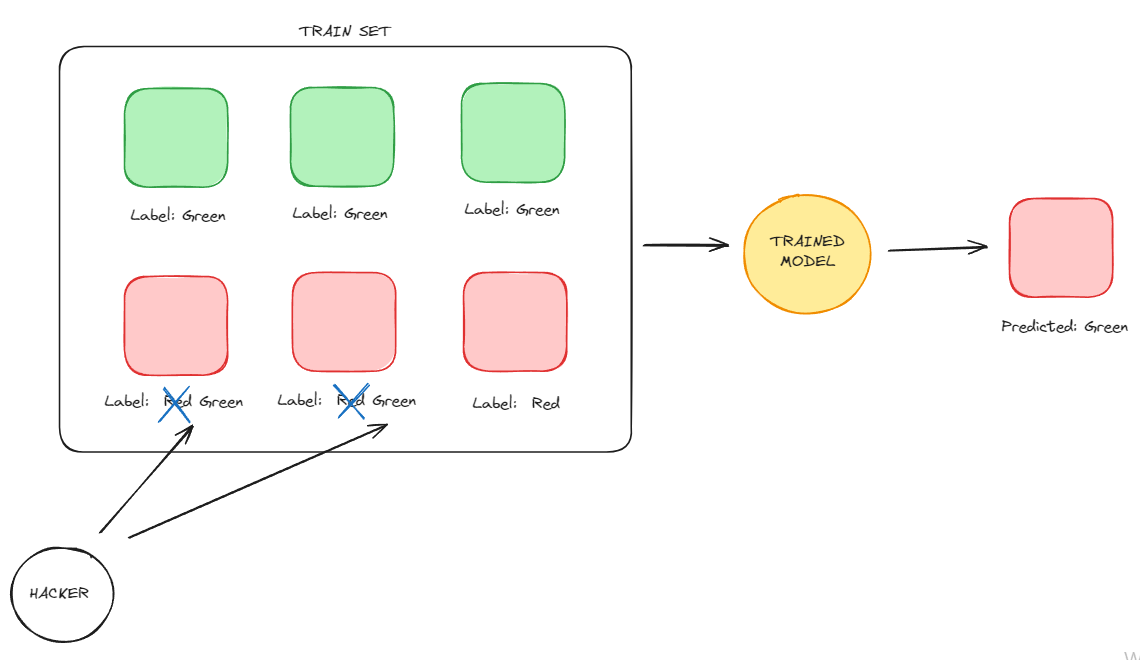
\includegraphics[width=0.8\textwidth]{images/ai_sec_poisoning_attack.png}
  \caption{Model Poisoning Example.}
\end{figure}

Model için kullanılacak eğitim veri setindeki verilerin güvenilir ve güvenli olduğundan emin olunmalıdır. Eğitim veri seti düzenli olarak denetlenmelidir. Eğitim veri güvenli bir şekilde saklanmalıdır. Yapay zeka modeli ve sistemleri, güvenlik testlerine tabi tutulmalıdır. 

\newpage

\subsection{Evasion}
Evasion saldırısı, sınıflandırma veya tanıma görevlerinde kullanılan modelin veri örneklerini manipüle ederek modelin yanlış kararlar almasını amaçlar. Saldırgan, modelin algılamasını veya sınıflandırmasını istenmeyen şekilde etkilemek için veri örneklerini manipüle eder. Örneğin beyaz renkli bir trafik işaretini kırmızı renge boyayarak yanlış tahmin yapmasına neden olabilir. Bu hileli örnekler, genellikle insan gözü ile fark edilemeyecek küçük şekilde değişiklikler içerebilir.
\begin{itemize}
    \item Saldırgan, görüntüye insan gözüyle farkedilmeyen değişiklikler yapar. (Image perturbation)
    \item Saldırgan, metin örneklerine işaretler veya eklemeler yapar.
\end{itemize}

\subsubsection{FGSM Method - Python Kodu}

\begin{lstlisting}[language=Python]
# FGSM Method
from art.attacks.evasion import FastGradientMethod
fgsm = FastGradientMethod(estimator=classifier, eps=0.2)
X_test_adversarial = fgsm.generate(x=X_test)
adv_pred = classifier.predict(X_test_adversarial)
adv_accuracy = calc_accuracy(adv_pred)
print(f"Accuracy after attack:{adv_accuracy * 100: .2f}")
\end{lstlisting}

\begin{figure}[h]
  \centering
  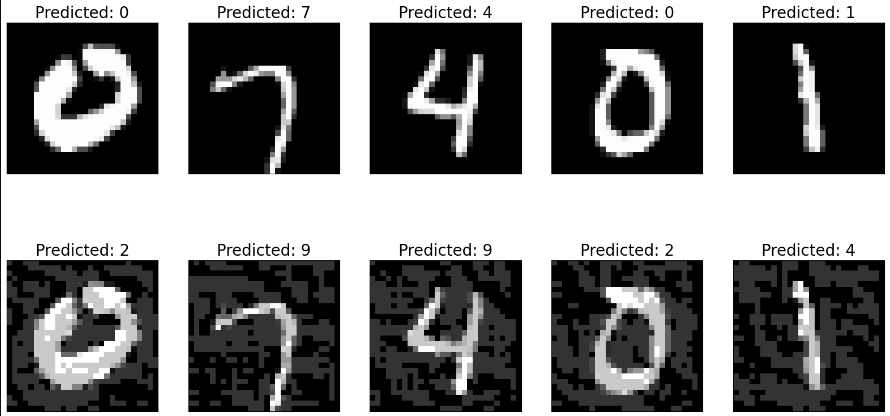
\includegraphics[width=0.8\textwidth]{images/evasion_fgsm.png}
  \caption{FGSM Attack Example.}
\end{figure}

\newpage

\subsubsection{Laser Beam Attack - Python Kodu}

\begin{lstlisting}[language=Python]
# Laser Beam Attack
from art.attacks.evasion.laser_attack.laser_attack import LaserBeamAttack
lb_attack = LaserBeamAttack(
    estimator = model,
    iterations = 50,
    max_laser_beam=(780, 3.14, 32, 32)
)
adv_images = []

for i in range(5):
    adv_image = lb_attack.generate(
        x=np.expand_dims(x_test[i], axis=0)
    )
    adv_images.append(adv_image)
\end{lstlisting}

\begin{figure}[h]
  \centering
  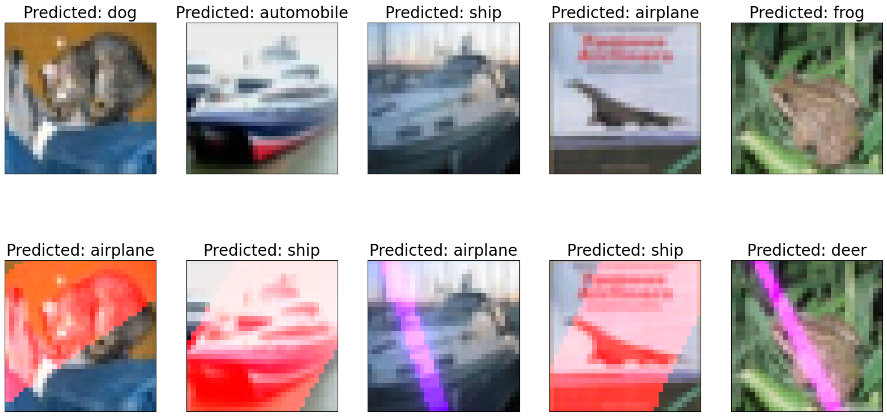
\includegraphics[width=0.8\textwidth]{images/evasion_laser_beam.png}
  \caption{Laser Beam Attack Example.}
\end{figure}

\newpage

\subsection{Membership Inference}
Membership Inference saldırısı, bir örneğin modelin eğitildiği veri setinde bulunup bulunmadığını belirlemeyi amaçlar. Sınıflandırma veya tanıma modelleri için kullanılır. Saldırgan, modelin tahmin ettiği sınıfların doğruluğunu ve modelin eğitim veri setindeki örnekleri tanıyıp tanımadığını değerlendirir.

\begin{figure}[h]
  \centering
  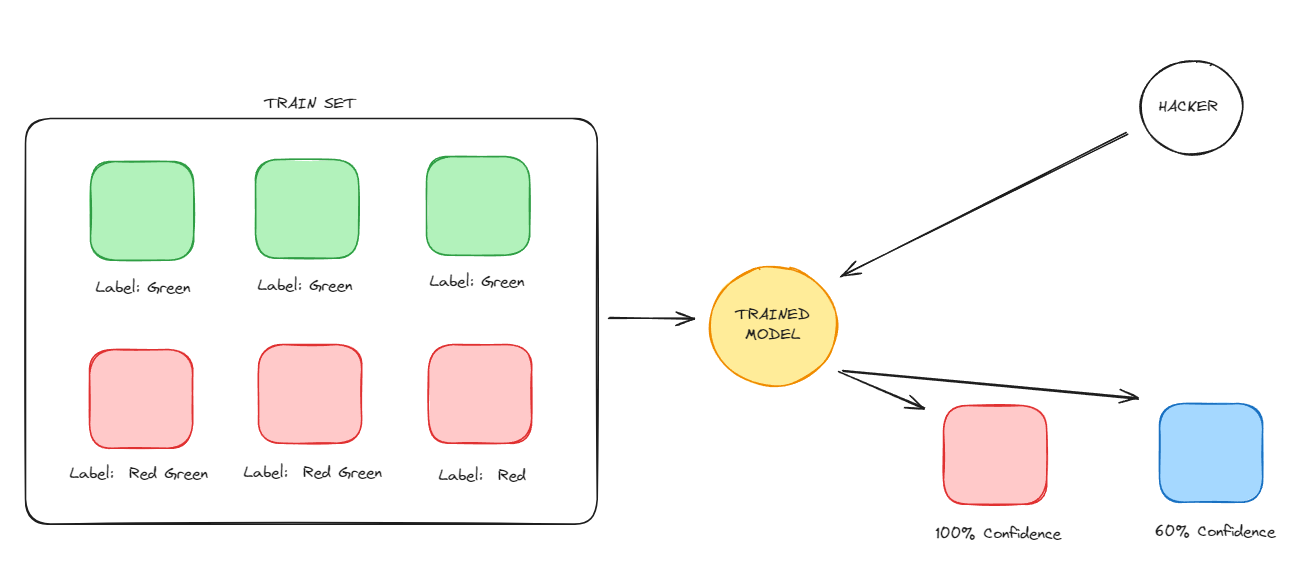
\includegraphics[width=0.8\textwidth]{images/ai_sec_membership_inference.png}
  \caption{Model Membership Inference Example.}
\end{figure}

\newpage

\subsection{Inversion}
Inversion saldırısı, modelin iç yapısını veya eğitim verisini ortaya çıkarmayı amaçlar. Giriş verilerine dayanarak modelin çalışma prensiplerini ve eğitim veri setini anlamayı amaçlar. Sınıflandırma veya tanıma modelleri için kullanılır.

\begin{figure}[h]
  \centering
  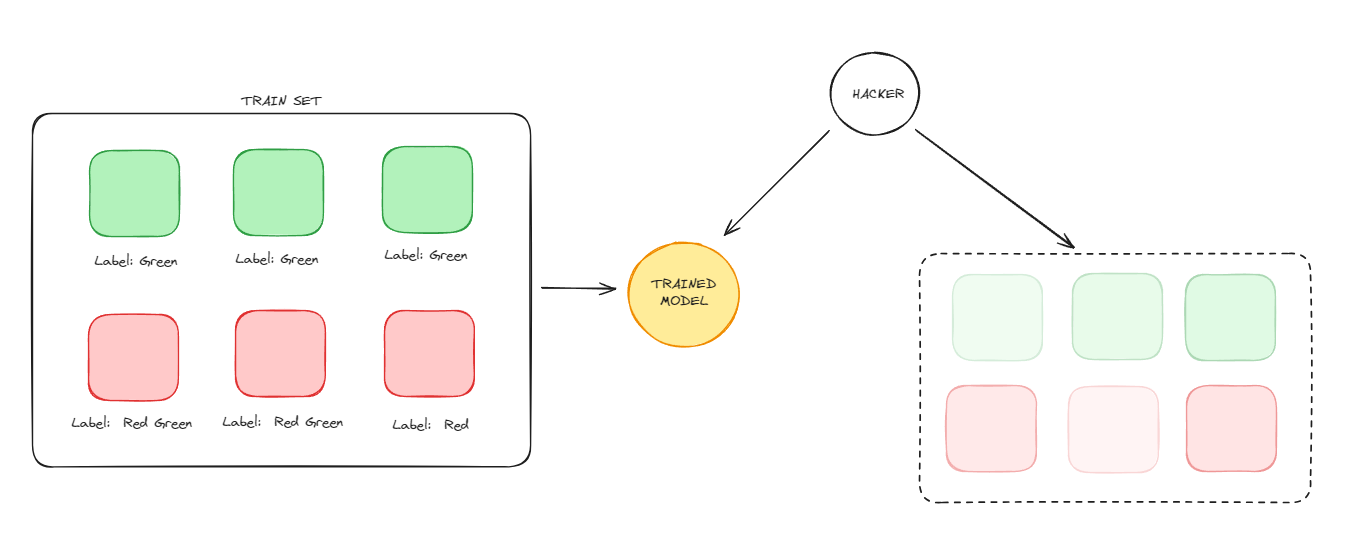
\includegraphics[width=0.8\textwidth]{images/ai_sec_model_inversion.png}
  \caption{Model Inversion Example.}
\end{figure}

\newpage

\subsection{Model Extraction}
Model Extraction (Model Theft), modelin mimarisini ve davranışını anlamak veya modeli yeniden oluşturmayı amaçlar. Saldırgan, modelin yapısını ve davranışlarını belirlemek için modeli sorgular. 

\newpage